\section{Conventional analysis}

  I have decided to conduct a conventional analysis to check whether we can find some regularities or anomalies that will help identifying groups of users using non-complex network methods.
  
  \subsection{Time oriented distribution of posts}
  
    First, I decided to have a look at the distribution of messages in topics during each year, month and hour during the day. The forum started in June 2001 and has had successively more messages posted per year for 6 consecutive years. Then it suddenly stopped and noted a significant, 32.36\% drop in message count in 2008. In this year, the United States of America, as well as pretty much the rest of the World, has suffered from major financial crisis. I never had access to the information about the \emph{page views}\footnote{Individual page impressions happening when users browse the website} of this particular message board, but I suspect that it might have been one of the reasons why an interest of the forum specialised in somewhat expensive equipment has decreased during that time. Figure \ref{fig:dist_year} shows the number of messages posted during each year of the data I have gathered (from June 21, 2006 to April 10, 2012).
    \begin{figure}[H]
      \centering
      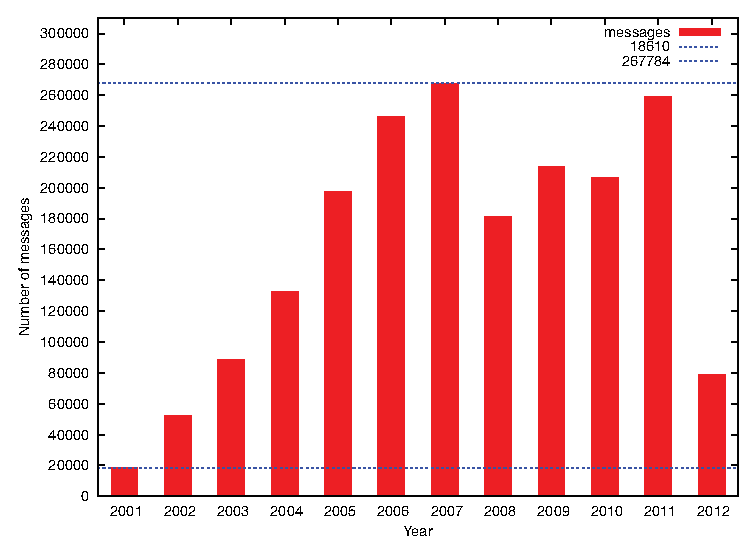
\includegraphics[width=\textwidth]{chapters/03_implementation/yearly}
      \caption{Message number distribution by year.}
      \label{fig:dist_year}
    \end{figure}
    
    Out of the curiosity I wanted to find out if I can confirm my suspicions by plotting the number of words related to prices against the total number of words. Figures \ref{fig:dist_price_year_1} and \ref{fig:dist_price_year_1} exhibit this ratio: the former, shown in full scale, and the latter \textquote{zoomed in} to exaggerate the peak usage that has happened during the year 2009. It may or may not be related to the Great Recession of 2009\footnote{D. Wessel from The Wall Street Journal (2010-04-08). \emph{Did \textquote{Great Recession} Live Up to the Name?} (available at http://online.wsj.com/article/SB10001424052702303591204575169693166352882.html) \\ C. Rampell from New York Times (2009-03-11). \emph{\textquote{Great Recession}: A Brief Etymology.} (available at http://economix.blogs.nytimes.com/2009/03/11/great-recession-a-brief-etymology/)} following the financial crisis of 2008. I will not follow on this topic any longer since this thesis is not about interpretation of the data from an economic standpoint.
    
    I do not think that it is possible to identify any groups of users here, other than those that registered early or not. Of course we could also try to extract the users that have signed up and did not post for some period of time or any other idea that can come to one's mind, but that information would not be very useful in my opinion.
    \begin{figure}[H]
      \centering
      \begin{subfigure}[H]{0.7\textwidth}
        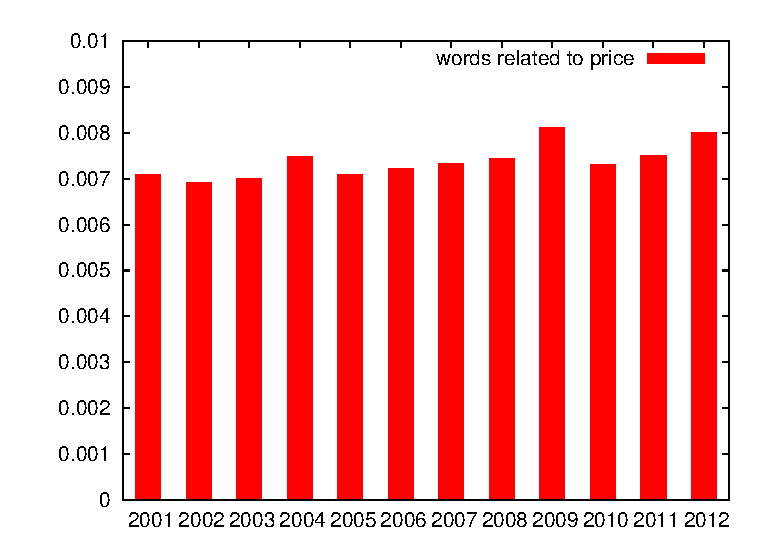
\includegraphics[width=\textwidth]{chapters/03_implementation/yearly_price1}
        \caption{Full scale.}
        \label{fig:dist_price_year_1}
      \end{subfigure}
      \\
      \begin{subfigure}[H]{0.7\textwidth}
        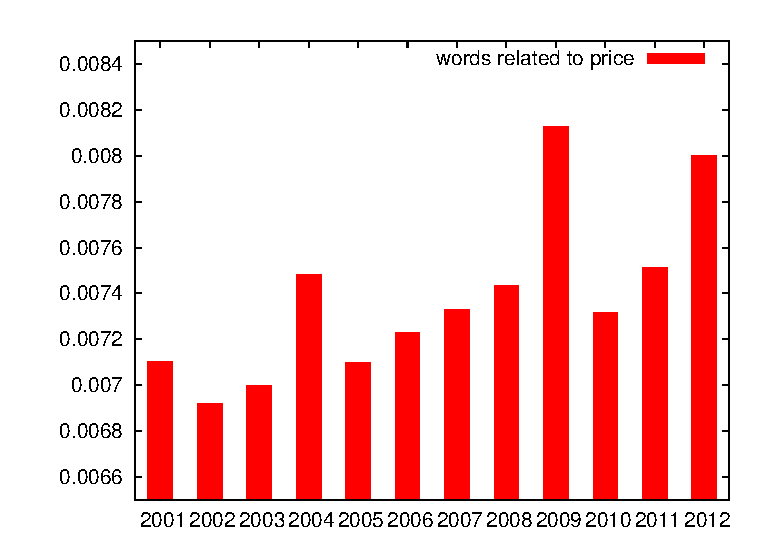
\includegraphics[width=\textwidth]{chapters/03_implementation/yearly_price2}
        \caption{Scale zoomed in.}
        \label{fig:dist_price_year_2}
      \end{subfigure}
      \caption{Ratio of the usage of words related to prices to the total number of words.}
      \label{fig:dist_price_year}
    \end{figure}
    
    Next, on figure \ref{fig:dist_month} we can see the distribution of messages grouped by month during which they were posted. One can clearly tell 4 peaks on January, February, March and December. I would account it to the fact that there is a \textquote{Christmas fever} period in December, where people are usually shopping for more gifts (so-called Christmas-gift-shopping patterns)\cite{FischerArnold1990,ArnoldReynolds2003}. The explanation for the several months following December could be fairly trivial, since these months are ideal for discussing recently obtained Christmas gifts. What would be interesting from this thesis standpoint is that we can at last identify a group of users that may be a target for potential marketing campains: people wanting to buy something.
    
    Days, or weeks immediately preceding and succeeding Christmas (or any other period of increased shopping) also seem to be the perfect time for malicious actions like advertorials\footnote{An advertisment in a form of an editorial.} or sponsored reviews.
    \begin{figure}[H]
      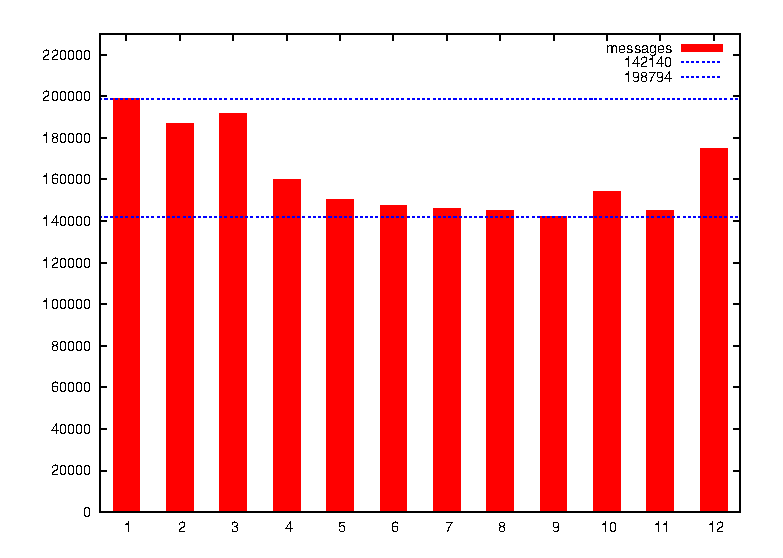
\includegraphics[width=\textwidth]{chapters/03_implementation/monthly}
      \caption{Message number distribution by month.}
      \label{fig:dist_month}
    \end{figure}
    
    The last figure in this section, figure \ref{fig:dist_hour} shows the distribution of messages posted throughout the day by the hour they were posted. The results do not seem to differ from the regular charts we see when analysing Internet traffic\cite{GebertPries2012}. The significantly lower number of messages posted during night hours is most likely related to the fact that, in general, people seem to sleep during this time of day\cite{Carskadon2002}. The number of messages in the night is huge anyway (it is around a half of the top number of messages during the day) which might indicate that the users of the forum are either very active or the community is international (i.e. located in different timezones). Otherwise, the night fluctuations would drift towards 0.
    
    I would not try to identify any particular groups of users based on the hours they post their messages at.
    \begin{figure}[H]
      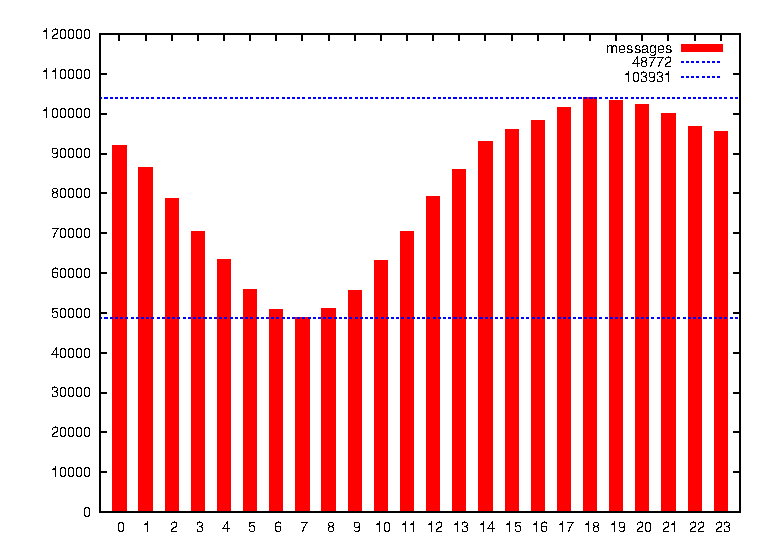
\includegraphics[width=\textwidth]{chapters/03_implementation/hourly}
      \caption{Message number distribution by hour.}
      \label{fig:dist_hour}
    \end{figure}